\section{Implementation details}
\label{sec:implementation-details}


\begin{figure}[t!]
\begin{center}
\includegraphics[width=.236\textwidth]{images/DD/snake_channel_060.png}
\includegraphics[width=.236\textwidth]{images/DD/snake_channel_180.png}
\includegraphics[width=.236\textwidth]{images/DD/snake_channel_320.png}
\includegraphics[width=.236\textwidth]{images/DD/snake_channel_540.png}
\end{center}
\caption{Free-surface simulation of water poured in a container with multiple interior walls causing the flow to meander around them. The frame shown in the right-most illustration corresponds to $114$ million active cells, in a $1024\times1024\times1024$ background grid.}
\label{fig:snake-channel}
\end{figure}

\textbf{Construction of adaptive operators} We construct the adaptively coarsened discretization of section \ref{sec:adaptive-approximation} based on a Galerkin
process. Let us consider the example of the finest level of the multigrid hierarchy. We define an interpolation operator $P^\ast_h$ that ``prolongates'' the adaptive
degrees of freedom $x^\ast$ into their trilinearly interpolated uniform counterparts $x=P^\ast_hx^\ast$ (this interpolation is conscious of any T-junctions). Thus,
the adaptive discretization of the Laplacian is simply computed as $A_h^\ast=(P^\ast_h)^TA_hP^\ast_h$. In fact, we never explicitly build the uniform matrix $A_h$,
but rewrite this equation as
$$
A_h^\ast=\sum_{a_{ij}\ne 0}a_{ij}\mathbf{p}_i\mathbf{p}_j^T
$$
where $a_{ij}=[A_h]_{ij}$, and $\mathbf{p}_k^T$ denotes the $k$-th row of $P^\ast_h$. This formulation allows us to construct the adaptive discretization directly
(by iterating over the uniform grid, and processing every spoke $a_{ij}$ of any stencil we encounter), without ever building the uniform matrix. Since our smoother
(Algorithm 2) never needs to use the \emph{uniform} subdomain discretization, we construct the adaptive discretizations of coarser levels of the hierarchy 
$A_h^\ast$, $A_{2h}^\ast$, $A_{4h}^\ast$, etc. by selective (Galerkin) coarsening of the immediately finer \emph{adaptive} discretization, rather than coarsening the
corresponding uniform discretization at that level into an octree.

\textbf{Avoiding nullspace issues} Global nullspace components (pockets of fluid with purely Neumann boundary conditions) are handled at the top-level PCG algorithm
via projection, as usual. In our smoother subroutine, we generally have the guarantee that the left-hand-side matrix $A_{\Gamma\Gamma}$ will be positive definite (it
is always symmetric), if the global matrix $A$ is definite too. However, it is possible for nullspace components to appear in the coarsened version of this matrix
$A_{\Gamma\Gamma}^{2h}$, $A_{\Gamma\Gamma}^{4h}$, as a result of the Galerkin procedure, in the vicinity of Neumann domain boundaries. To avoid this, we slightly
shift the eigenvalues of every coarsened discretization, say $A_{2h}^\ast$ by adding a minute multiple of the identity. The shifted matrix $A_{2h}^\ast+\epsilon I$
is practically spectrally equivalent to the original, and fully appropriate as a substitute in a multigrid hierarchy. Since we use direct solvers to invert
$A_{\Gamma\Gamma}$ in the smoother, conditioning is not an issue. Effectively, this eigenvalue shift will penalize solution components that lie in the nullspace to
be effectively equal to zero.

\textbf{Boosting accuracy} We use a high-order defect correction technique \cite{trottenberg:2001:multigrid} to allow our approximate inverse of a first-order
discretization to be used as a CG preconditioner for a higher order scheme. We structure our top-level PCG solver to implement matrix-vector multiply operations in
accordance with a second order accurate discretization of the Laplace operator \cite{Enright:2003:UTP}. Upon invocation of the preconditioner, however, we perform
the following steps: (i) We execute a few iterations of a Jacobi smoother, using the 2nd order operator, (ii) we then compute the residual, and multiply this with
our first-order preconditioner, and finally (iii) we again compute the residual $r$, write the error equation $Ae=-r$ using the second order operator, which we solve
using the same number of Jacobi iterations. We finally add the correction back to the result returned by the preconditioner. This operation, as described, preserves
the symmetry and definiteness of the preconditioner, and allows the first order method to be used as an effective preconditioner for the second-order problem (at the
comparably minimal expense of some additional smoothing effort near the high-order interface).

\textbf{Sparse grid storage}
 We used an ad-hoc sparse grid data structure to hold our grid data, for all
our examples which utilized highly irregular, sparsely populated grids.
 Our data structure partitions a virtual enclosing grid into rectangular blocks (of typical size $8^3$ voxels, in our examples), and stores them in a linearized array,
maintaining explicit pointers to the $26$ neighboring blocks to facilitate traversal during kernel invocation. This representation is reflected in both our CPU and GPU/Xeon Phi
implementations of all performance-sensitive kernels.

\begin{figure}[h]
\begin{center}
\includegraphics[width=0.48\columnwidth]{images/DD/convergence_plot.png}
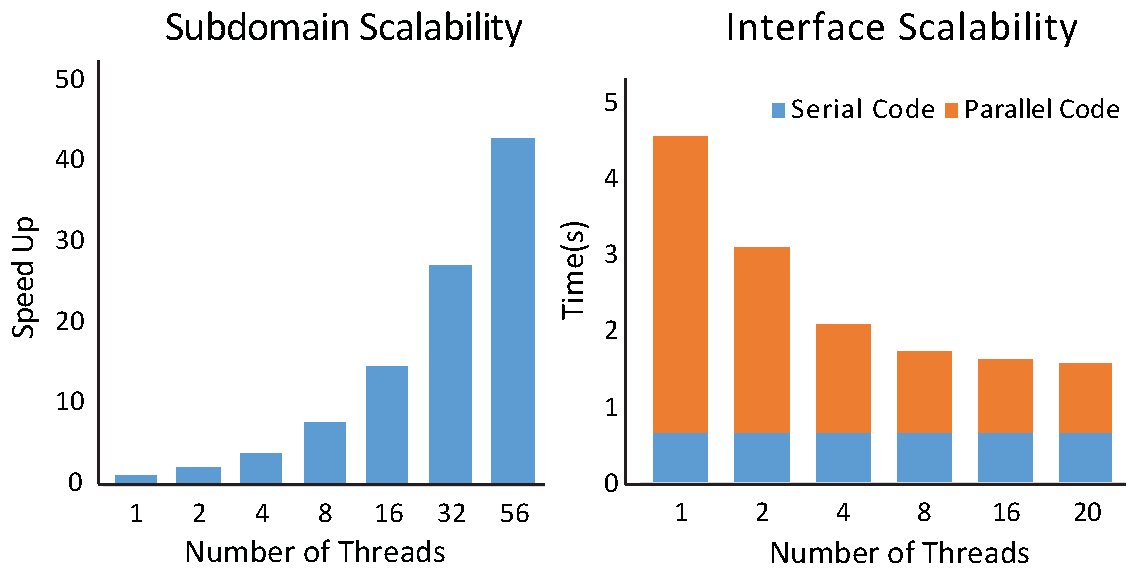
\includegraphics[width=0.48\columnwidth]{images/DD/scalability.pdf}
\end{center}
\caption{
\changed{(Top) convergence profiles for ICPCG, MCPCG and DDPCG (our method) from the water simulation of Figure \ref{fig:snake-channel}. The numbers ($B$-$I$-$B$) indicate
  multigrid smoothers that perform $B$ boundary sweeps, then $I$ interior sweeps, and $B$ more boundary sweeps at the end. V-Cycle counts in DDPCG reflect the number of cycles
  used in the approximate solution of each subdomain. (Bottom) Scaling of subdomain solvers (left; on Xeon Phi) and interface solver (right; on CPU) relative to the active cores/threads utilized.}
{ Convergence profiles for ICPCG, MGPCG (1 V-cycle, 3 boundary and 1 interior smoothing iteration), MGPCG (1 V-cycle, 7 boundary and 1 interior smoothing iteration), DDPCG (2
  V-cycles per subdomain, 3 boundary and 1 interior smoothing iteration), and DDPCG (3 V-cycles per subdomain, 7 boundary and 1 interior smoothing iteration).}
}
\label{fig:convergence-profiles}
\end{figure}


\section{Incompressible free surface flow}
\label{sec:free-surface}

We solve the incompressible Euler equations
$$
\vec{\boldsymbol{u}}_t+(\vec{\boldsymbol{u}}\cdot\nabla)\vec{\boldsymbol{u}} + \frac{\nabla p}{\rho} = \vec{\boldsymbol{f}}, \hspace{.4in}
\nabla\cdot\vec{\boldsymbol{u}} = 0
$$
using the splitting scheme as described in~\cite{Stam:1999:StableFluids}. Here,
$\vec{\boldsymbol{u}}=(u,v,w)$ is the velocity field vector, $\rho$ is the
fluid density, $p$ is the scalar pressure field, and
$\vec{\boldsymbol{f}}$ denotes external forces (such as gravity).
We discretize these equations on a MAC grid, where we first explicitly update
the advection terms
$$
\label{eqn:advection}
\frac{\vec{\boldsymbol{u}}^\star-\vec{\boldsymbol{u}}^n}{\Delta t}+(\vec{\boldsymbol{u}}\cdot\nabla)\vec{\boldsymbol{u}} = \vec{\boldsymbol{f}}
$$
using a semi-Lagrangian scheme~\cite{Selle:2008:MacCormack} and then solve for the
pressure via a Poisson equation
$$
\nabla\cdot\frac{\nabla p}{\rho}=\frac{\nabla\cdot\vec{\boldsymbol{u}}^\star}{\Delta t}
$$
in order to update the intermediate velocity as follows
$$
\frac{\vec{\boldsymbol{u}}^{n+1}-\vec{\boldsymbol{u}}^\star}{\Delta t}+\frac{\nabla p}{\rho}=0
$$
For tracking the free surface, we generally follow~\cite{Enright:2002:ARC} using the
level set advection of~\cite{Enright:2005:FAS}, the
reinitialization scheme of~\cite{Losasso:2005:SATLMIF}, velocity extrapolation method of~\cite{Adalsteinsson:1999:FCEVLS},
and a second order accurate pressure discretization of~\cite{Enright:2003:UTP}.

\begin{figure*}[t]
\begin{center}
\includegraphics[width=.240\textwidth]{images/DD/dragons_028.png} \includegraphics[width=.240\textwidth]{images/DD/dragons_050.png} \includegraphics[width=.240\textwidth]{images/DD/dragons_115.png} \includegraphics[width=.240\textwidth]{images/DD/dragons_220.png}
\end{center}
\caption{Water poured in a pool with multiple immersed objects. Second figure from the right shows $70$M  active cells, in a $1024^2\!\times\!512$ grid.}
\label{fig:free-surface-flow}
\end{figure*}
